%!TEX root = origin.TEX
\chapter{Introducción}
	\pagenumbering{arabic}
	\setcounter{page}{1}
	\renewcommand{\baselinestretch}{1} %doble espacio paratodo el texto
	Al conducir en carreteras congestionadas, a veces es difícil mantener los ojos en todas partes a la vez, comprobando el camino por delante, el tráfico venidero, lo que está detrás de usted, tratar de mantener su velocidad; es por ello, que existen mecanismos destinados a reglamentar el tránsito, advertir o informar a los usuarios mediante palabras, sonidos o símbolos determinados. Un claro ejemplo de ello, es la policía de tránsito o las señalizaciones vehiculares que según sea el caso, en todos los países regulan el tránsito e informan al usuario sobre direcciones, rutas, destinos, así como dificultades existentes en las carreteras y previenen cualquier peligro que podría presentarse en la circulación vehicular.

	\vskip 0.15cm
	Sin embargo, cuando estos mecanismos no son conocidos o percibidos pueden ocasionar no solo que la congestión del tráfico aumente, sino que también se produzcan accidentes que en muchos casos derivan en consecuencias fatales, generando inseguridad vial.

	\vskip 0.15cm
	La inseguridad vial es un problema de interés mundial, según el último informe de la OMS (Organización Mundial de la salud) anualmente cerca de 1,3 millones de personas mueren alrededor del mundo y entre 20 y 50 millones padecen traumatismos no mortales \citep{OMS}. Esto representa la segunda de las principales causas de muerte a nivel mundial entre los jóvenes de 5 a 29 años de edad, y la tercera entre la población de 30 a 44 años. Son distintas las causas que conllevan a este problema, de las cuales las principales pueden ser la falta de concientización y educación vial. 
	
	\vskip 0.15cm	
	Es un problema para la economía mundial de los países, así también para los hogares. A pesar de ello, se invierte muy poco dinero en prevenir los accidentes y las lesiones causadas por el tránsito. El sector salud se beneficiaría mucho de una mejor prevención de las lesiones porque se reducirían las hospitalizaciones y la gravedad de los traumatismos \citep{CNSV}.

	\vskip 0.15cm
	Los usuarios vulnerables de la vía pública representan la mitad de todas las muertes por accidente de tránsito a nivel mundial y es mayor en países de ingresos bajos, siendo la causa principal, el aumento de velocidad durante la conducción de los vehículos \citep{OMS}.

	\vskip 0.15cm
	\begin{figure}[H]
	\begin{center}
	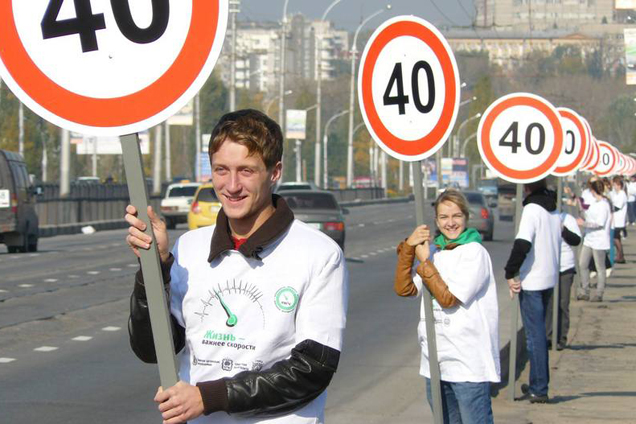
\includegraphics[width=0.5\textwidth]{images/intro/velocidad}
	\end{center}
	\begin{center}
	\caption{\small{Señalización de velocidad}}
	{\small{Fuente: \cite{OMS}}}
	\end{center}
	\vspace{-1.5em}
	\end{figure}
	
	Por otra parte, de los vehículos que se venden en el 80\% de los países no cumplen las normas básicas de seguridad, es por ello que se debe trabajar en obtener vehículos más seguros ya que es un factor fundamental para prevenir de alguna forma los accidentes de tránsito o reducir la probabilidad de traumatismos graves en caso de que estos se produzcan \citep{OMS}.
	
	\vskip 0.15cm
	En lo que respecta al sector nacional, es decir en el Perú, la inseguridad vial es un problema constante ya que los peruanos mueren más por los accidentes de tránsito que por la inseguridad ciudadana según datos mostrados por María Edith Baca de la Organización Panamericana de la Salud \citep{OPS}. Adicionalmente, según un estudio realizado por RPPData en base a reportes de la Policía publicados entre el 2010 y el 2016, en el país cada día fallecen 8 personas en accidentes de tránsito, \citep{RPPData}. El costo de estas muertes, calculado en S/ 19,165 millones por la consultora Alauda especializada en mantenimiento de infraestructura, representó un 3.1\% del PBI \citep{Gestion2}.  
	
	
	\vskip 0.15cm
	En el 2016 se obtuvo un índice Global de Satisfacción del Conductor \citep{CNN} en el cual, Perú y la capital Lima se encuentran respectivamente en la lista de peores países y ciudades para conducir en América Latina, esto se ve reflejado en que los últimos años se ha incrementado el índice de mortandad originados por los accidentes de tránsito siendo las principales causas de los mismos el exceso de velocidad, estado de ebriedad del conductor, imprudencia temeraria y el desacato a las señales de tránsito, todas ellas de responsabilidad directa del conductor del vehículo motorizado al no respetar las señales de tránsito\citep{SUTRAN}. 
	
	\begin{figure}[H]
	\begin{center}
	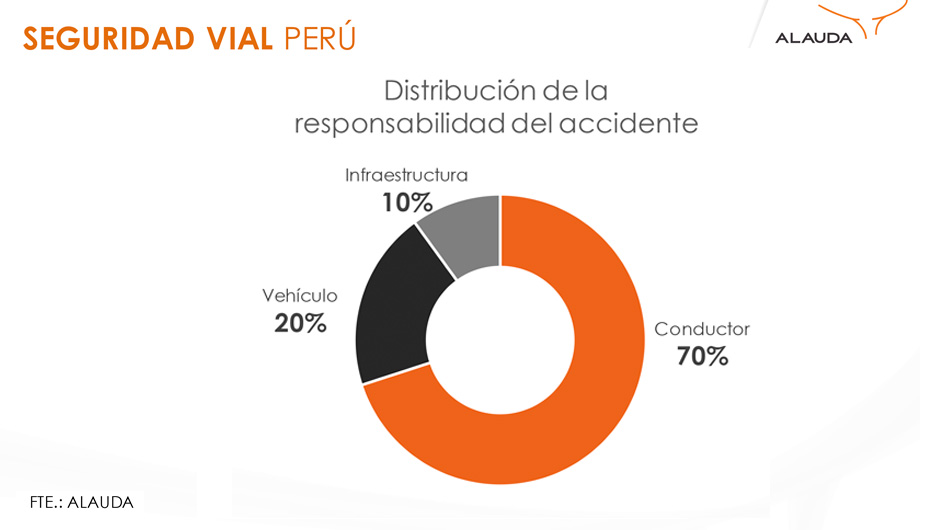
\includegraphics[width=0.5\textwidth]{images/intro/responsabilidad_cond}
	\end{center}
	\begin{center}
	\caption{\small{Análisis de responsabilidad de accidentes}}
	{\small{Fuente acceso: \cite{Gestion1}}}
	\end{center}
	\vspace{-1.5em}
	\end{figure}

	\begin{figure}[H]
	\begin{center}
	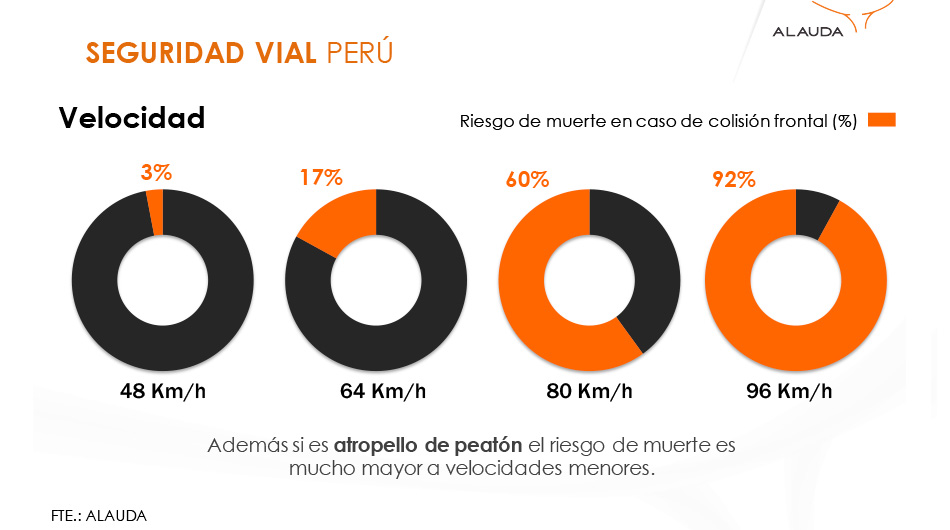
\includegraphics[width=0.6\textwidth]{images/intro/velocidad_ind}
	\end{center}
	\begin{center}
	\caption{\small{Influencia de velocidad en accidentes}}
	{\small{Fuente acceso: \cite{Gestion1}}}
	\end{center}
	\vspace{-1.5em}
	\end{figure}
	
	%Aunque se han publicado algunos estudios sobre este tema, aún no existen comparaciones sistemáticas de enfoques que sean imparciales y no se dispone de conjuntos de datos de referencia completos. 
	
	El reconocimiento de estas señales es un problema de clasificación multi-categórica que comúnmente presenta desigualdades en las frecuencias de aparición de sus clases. Además, las señales de tránsito muestran una amplia gama de variaciones entre las clases en términos de color, forma y la presencia de símbolos, leyendas o texto. Además, existen subconjuntos de clases (por ejemplo, signos de límite de velocidad) que son muy similares entre sí, lo que representa un reto para un reconocedor  automático, el cual tiene que hacer frente a grandes variaciones en las apariencias visuales debido a cambios de iluminación, oclusiones parciales, rotaciones, condiciones meteorológicas, escalamiento, etc.
    

	
\section{Justificación de la investigación} 

	\subsection{Justificación Académica}

	Recientemente las redes convolucionales profundas han superado los métodos tradicionales de aprendizaje en la clasificación de imágenes. Con los rápidos avances de las estructuras de algoritmos de aprendizaje profundo y la factibilidad de su implementación de alto rendimiento con unidades de procesamiento gráfico (GPU), es ventajoso investigar en problemas de clasificación de imágenes desde la perspectiva de un aprendizaje profundo eficiente. Sin embargo, realizar esto no es tarea simple, ya que se requiere de un modelo de reconocimiento que funcione para imágenes que se encuentran comúnmente influenciadas por la iluminación, la orientación, la variación de velocidad de los vehículos, entre muchos otros problemas más.  \vskip 0.2cm

	En este sentido, esta investigación pretende la elaboración de un modelo basado en el aprendizaje profundo de redes convolucionales que permita el reconocimiento de señales de tránsito vehicular. La siguiente figura muestra un diagrama de bloques con la secuencia de actividades que demanda el reconocimiento.

	\begin{figure}[H]
	\begin{center}
	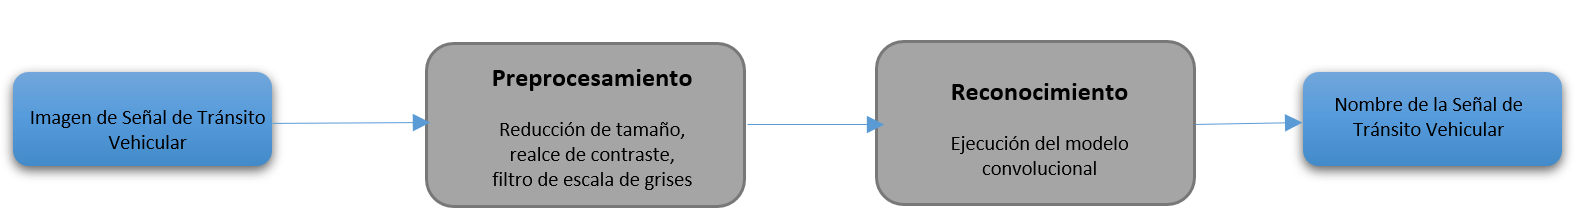
\includegraphics[width=0.8\textwidth]{images/intro/bloque}
	\end{center}
	\begin{center}
	\caption{\small{Diagrama de bloques para el reconocimiento}}
	{\small{Fuente: Elaboración propia}}
	\end{center}
	\vspace{-1.5em}
	\end{figure}


	Por lo tanto, la importancia de esta investigación en el punto de vista de ciencias de la computación se justifica en poner en práctica los conocimientos adquiridos en la formación académica, siendo los más resaltables el tema de procesamiento de imágenes e inteligencia artificial con la finalidad de obtener un modelo robusto de redes neuronales convolucionales basadas en el aprendizaje profundo (deep learning) que permita analizar el contenido de imágenes para el reconocimiento de señales de tránsito vehicular. 


	\subsection{Justificación Social}
	
	Teniendo conocimiento de lo descrito al inicio de este capítulo, la visibilidad y conocimiento de señales de tráfico es crucial para la seguridad de los conductores y es por ello que la introducción de un modelo de reconocimiento de señales de tránsito que funcione en diferentes contextos puede formar parte de la solución a que se puedan evitar constantes infracciones y muertes, y en consecuencia reducir estos índices progresivamente. Por ejemplo, el reconocimiento de estas señales en el momento de la conducción puede ofrecer la posibilidad de dar una notificación al no darse cuenta de un cambio en el límite de velocidad, el aviso de que se está cometiendo una infracción al girar o estacionarse donde no se debe o la advertencia de un peligro potencial por delante. Por otro lado, cuando usuarios desconocen de alguna señal de tránsito, una aplicación móvil que dé la posibilidad de reconocer automáticamente aquella señal serviría como aporte en la educación vial.\vskip 0.2cm

	Por lo tanto, esta investigación es importante porque a través de un modelo que reconozca señales de tránsito vehicular se podría contribuir en la industria automotriz, específicamente en los sistemas avanzados de asistencia al conductor (del inglés, \textit{ADAS}); así como también se ha descrito anteriormente, el modelo pretendido puede ser usado en diferentes plataformas y formar parte de diversos mecanismos que buscan dar soluciones a la inseguridad vial. \vskip 0.2cm
	
	Todos los hechos descritos hacen que el reconocimiento de las señales de tránsito sea un reto desafiante y esencial en muchos aspectos, no solo para contribuir en los esfuerzos de la industria automotriz en el campo de la asistencia al conductor, sino también incluso para organismos gubernamentales quienes se dan cuenta de la problemática que representa la inseguridad vial y buscan constantemente introducir nuevos mecanismos y tecnologías que faciliten y mejoren la conducción vehicular para el beneficio propio del conductor y en general para la seguridad vial en la sociedad.


\section{Formulación del problema}

  En este trabajo, se propone discutir el modelo de redes neuronales convolucionales basado en el problema del reconocimiento de imágenes para responder a la siguiente pregunta:
 \begin{center} 
     ¿Cómo se puede reconocer de manera automática señales de tránsito vehicular?
 \end{center}

\section{Hipótesis}
	 Un modelo basado en el aprendizaje profundo de redes neuronales convolucionales permitirá el reconocimiento automático de señales de tránsito vehicular.



\section{Objetivos}
	\subsection{Objetivo general}
	La investigación tiene por objetivo principal implementar un modelo basado en el aprendizaje profundo de redes neuronales convolucionales para reconocer automáticamente señales de tránsito vehicular.
	
	\vskip 0.2cm
		
	\subsection{Objetivos específicos}
	\begin{enumerate}
	
	\item[a)] Obtener un conjunto de imágenes(dataset) donde se muestren diferentes señales de tránsito vehicular.
	\item[b)] Dividir un conjunto de imágenes 3 grupos, uno para el entrenamiento, uno para validación del entrenamiento y un tercero para evaluación del modelo. 
	\item[c)] Analizar el dataset de entrenamiento a través de métodos de procesamiento de imágenes. De ser necesario, con estos mismos, aumentar la cantidad de imágenes.
	\item[d)] Implementar diferentes arquitecturas de redes convolucionales profundas en las cuales el dataset de entrenamiento será procesado.
	\item[e)] Experimentar el uso de diversas funciones de activación, funciones de costo, ajuste de hiperparámetros y métodos de optimización para dichas arquitecturas. 
	\item[f)] Evaluar individualmente el rendimiento que se obtiene de las arquitecturas implementadas en el dataset de entrenamiento y evaluación.
	\item[g)] Elaborar un modelo computacional basado en las evaluaciones realizadas.
	\end{enumerate}



\section{Estructura de la tesis}

	\vskip 0.1cm
	El presente trabajo está dividido en cinco capítulos. El primer capítulo presenta los aspectos generales de la investigación realizada tal como justificación, formulación del problema, hipótesis, los objetivos y la estructura de la tesis.

	El capítulo describe los materiales y las técnicas de recolección de datos, se presenta el referencial teórico, soporte del tema, contemplando los conceptos de inteligencia artificial, aprendizaje automático basado en redes neuronales detallando y diferenciando sus características en el área de aprendizaje profundo. Además, se analiza las características y procesos de una red convolucional a detalle. Finalmente se describe el método empleado durante la investigación.

	En el tercer capítulo es el desarrollo de la tesis, diseñándose los modelos propuestos y explicando la implementación de cada uno de ellos.
	
	En el cuarto capítulo se presentan los resultados y discusión obtenidos en la investigación.

	En el capítulo cinco se presentan las consideraciones finales obtenidas en esta tesis. Inicialmente se presentan las conclusiones, seguida de las recomendaciones para futuras investigaciones relacionadas al tema en cuestión.

	Finalmente, se describen las referencias bibliográficas usadas para la investigación en esta tesis y los anexos donde se presentan pseudocódigos de los programas elaborados.

